\documentclass[12pt]{article}
\usepackage{calc}
\usepackage{tikz}
\usetikzlibrary{arrows,decorations.markings}
\tikzstyle{vertex}=[circle, draw, inner sep=0pt, minimum size=18pt]
\newcommand{\vertex}{\node[vertex]}
\newcounter{Angle}

\pagestyle{empty}
\begin{document}
{\large\bf
\[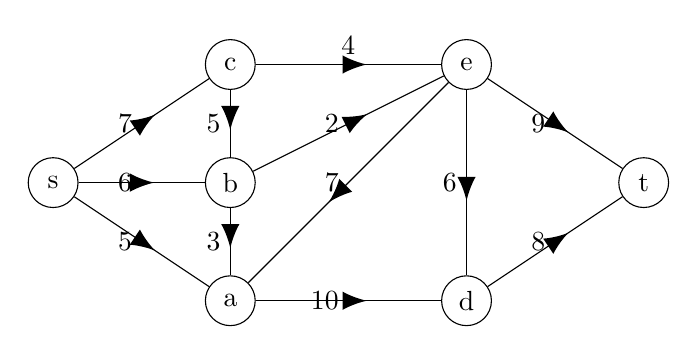
\begin{tikzpicture}[x=1.5cm, y=1.5cm
    ,every edge/.style={
        draw,
        postaction={decorate,
                    decoration={markings,mark=at position .6 with
		    {\arrow[line width=2pt,black]{latex}}} } }
]
\vertex (s) at (.5,0) {s};
\vertex (a) at (2,-1) {a};
\vertex (b) at (2,0)  {b};
\vertex (c) at (2,1)  {c};
\vertex (d) at (4,-1) {d};
\vertex (e) at (4,1)  {e};
\vertex (t) at (5.5,0) {t};
\path
(s) edge node [below,left] {5} (a) 
    edge node [below,left] {6} (b) 
    edge node [above,left] {7} (c) 
(a) edge node [above,left] {10} (d)
(b) edge node [above,left] {3} (a) 
    edge node [above,left] {2} (e) 
(c) edge node [above]      {4} (e)
    edge node [above,left] {5} (b) 
(d) edge node [above,left] {8} (t)
(e) edge node [above,left] {7} (a) 
    edge node [above,left] {6} (d) 
    edge node [above,left] {9} (t)
;
\end{tikzpicture}\]
}\end{document}
